%%%%%%%%%%%%%%%%%%%%%%%%%%%%%%%%%%%%%%%%%%%%%%%%%%%%%%%%%%%%%%%%
%% SECTION Analysis of Optimal Designs --- Vanishing Model Error
%%%%%%%%%%%%%%%%%%%%%%%%%%%%%%%%%%%%%%%%%%%%%%%%%%%%%%%%%%%%%%%%
\section{Characterization of D-Optimal Designs with Vanishing Model Error}\label{section:vanishing}
We now turn to analyze D-optimal designs when $\modcov = 0$. Our goal
is to prove Theorem \ref{thm:char} --- a characterization of D-optimal
designs.


%% \subsection{The Nonlinear Eigenvalue Problem}\label{subsec:eigenproblem}
The necessary first-order condition for D-optimality summarized in
Theorem \ref{thm:constrained}, when $\Sigma= \sigma^2I$ (i.e. when
$\modcov = 0$) becomes
\begin{equation}\label{eq:eigenproblem}
  \sigma^{-2}\fwd \postcov \fwd^* \obs^* = \obs^* \Xi,
\end{equation}
with $\Xi$ diagonal. We think of \eqref{eq:eigenproblem} as an
eigenvalue problem for the self-adjoint operator $\sigma^{-2}\fwd
\postcov \fwd^*$, where rows of $\obs$, namely $\meas_j,j=1,\dots, m$,
are eigenvectors. However, $\postcov$ depends on $\obs$ and thus, we
refer to \eqref{eq:eigenproblem} as a \emph{nonlinear} eigenvalue
problem. The following Proposition and Lemma are proved in the
appendix:

\begin{restatable*}[Two applications of Woodbury Matrix Identity]{proposition}{woodbury}\label{prop:twice woodbury}
  Assume $\fwd \prcov \fwd^*$ is invertible. Then
  \begin{align*}
    \begin{split}
      \fwd( \prcov^{-1} + \sigma^{-2}  \fwd^* \obs^* \obs \fwd )^{-1} \fwd^* 
      %
      %
      = \left ( (\fwd\prcov\fwd^*)^{-1} + \sigma^{-2}  \obs^* \obs \right )^{-1},
    \end{split}
  \end{align*}  
\end{restatable*}

\begin{restatable*}[Simultaneous diagonizability]{lemma}{simdiag}\label{lemma:sim diag}
  Let $\hil$ separable Hilbert space, $C:\hil \to \hil$ self-adjoint
  and $\func_1,\dots,\func_m \in \hil$. Denote $\func^*$ the element
  $\func$ acting as a linear functional. If
  \begin{equation*}
   (C + \sum_{j=1}^m \func_j\func_j^*) \func_l = \xi_l \func_l,\ l = 1,\dots,m
  \end{equation*}
  then $C$ and $\sum_{j=1}^m \func_j \func_j^*$ are simultaneously
  diagonalizable.
\end{restatable*}

\begin{proposition}[Eigenvectors of a D-optimal design]\label{prop:same ev}
  Let $\obs$ satisfy the nonlinear eigenvalue problem
  \eqref{eq:eigenproblem}. Then $\obs^*\obs$ has the same eigenvectors
  as $\fwd \prcov \fwd^*$.
\end{proposition}
\begin{proof}
  \begin{align}\label{eq:mod conditions}
    \begin{split}
      \obs^* \Xi &= \sigma^{-2}\fwd \postcov \fwd^* \obs^*  \text{ (by \eqref{eq:eigenproblem})}\\
      %
      %
      %
      &= \sigma^{-2} \fwd( \prcov^{-1} + \sigma^{-2}  \fwd^* \obs^* \obs \fwd )^{-1} \fwd^* \obs^*  \text{ (by \eqref{eq:postcov})} \\
      %
      %
      %
      &= \sigma^{-2} \left ( (\fwd\prcov\fwd^*)^{-1} + \sigma^{-2}  \obs^* \obs \right )^{-1} \obs^* \text{ (by Proposition \ref{prop:twice woodbury})}.
    \end{split}
  \end{align}

  Now take $\func_j^{*} = \meas_j$ and $C := (\fwd \prcov
  \fwd^*)^{-1}$ and use Lemma \ref{lemma:sim diag}.
\end{proof}

Since we made no assumption regarding the ordering of $\{\lambda_i\}$,
we can denote the corresponding non-zero eigenvalues of $\obs^*\obs$
by $\{\eta_i\}_{i=1}^{k}$ and let $\eta_i = 0$ for $i \geq k+1$.

\begin{proposition}\label{prop:true target}
  Let $\obs$ with $m$ observations satisfy the nonlinear eigenvalue
  problem \eqref{eq:eigenproblem}. Let $\{\eta_i\}_{i=1}^{\infty}$
  eigenvalues of $\obs^*\obs$ and $\{\lambda_i\}_{i=1}^{\infty}$ the
  corresponding eigenvalues of $\fwd \prcov \fwd^*$. Let $k:=\rank
  \obs^*\obs$. Without loss of generality, let $\eta_i > 0$ for $i\leq
  k$ and $\eta_i = 0$ for $i > k$. Then:
  \begin{enumerate}
    \item $k \leq m$ and $\obs^*\obs$ has exactly $k$ positive
      eigenvalues.
    \item
      \begin{equation*}
        \tar(\obs) = \frac12 \sum_{i=1}^{k} \log (1 + \sigma^{-2}\lambda_i\eta_i) = \frac12 \sum_{i=1}^{m} \log (1 + \sigma^{-2}\lambda_i\eta_i).
      \end{equation*}
    \item Let $\obs$ a D-optimal design. Then $\eta_i > 0$ for
      eigenvectors corresponding to the $k$ largest $\lambda_i$.
  \end{enumerate}
\end{proposition}
\begin{proof}
  Part (1) is trivial. To see part (2) holds: 
  \begin{align}
    \begin{split}
      \tar(\obs) &= \frac12\log \det \left (I + \sigma^{-2} \prcov^{1/2} \fwd ^* \obs^*
      \obs \fwd \prcov^{1/2}\right )\\% \text{ (by definition)}\\
      %
      &= \frac12 \log \det \left (I + \sigma^{-2} \obs^* \obs \fwd
      \prcov\fwd^* \right ) \text{ (Sylvester's Determinant
      Theorem)}\\
      %
      %
      %
      &=\frac12 \log \prod_{i=1}^{\infty} ( 1 + \sigma^{-2} \lambda_i\eta_i ) \text{ (Proposition \ref{prop:same ev})} \\
      %
      %
      %
      %&=\frac12 \log \left ( \prod_{i=1}^{k} ( \lambda_i^{-1} + \sigma^{-2} \eta_i )\prod_{i=1}^{k} \lambda_i \right )
      %
      %
      %
      &=\frac12 \sum_{i=1}^{k} \log (1 + \sigma^{-2}\lambda_i\eta_i). 
      %
      %
      %% &=\frac12 \sum_{i=1}^{k} \log(\sigma^2\lambda_i^{-1} + \eta_i) - k\log \sigma + \frac12\sum_{i=1}^k \log \lambda_i.
    \end{split}
  \end{align}
  Part (3) holds since $\log$ is increasing and $\eta_i \geq 0$.
\end{proof}


\begin{proposition}\label{prop:kkt}
  Let $\tar: \mathbb{R}^m \to \mathbb{R}$, $\psi(\eta) =
  \frac{1}{2}\sum_{i=1}^m \log (1+\sigma^{-2}\lambda_i \eta_i)$, with
  $\lambda_i > 0$ and $\sigma^{2} > 0$. Then the maximum of $\tar$
  subject to $\eta_i \geq 0$ and $\sum\eta_i = m$ is obtained at
  \begin{equation}
  \eta_i = \begin{cases}
    \frac{m}{k} - \sigma^2 \lambda_i^{-1} + \sigma^2 \frac{1}{k} \sum_{j\in A} \lambda_j^{-1} & i \in A \\
    0 & i \in A^c
  \end{cases}
  \end{equation}
  where $A:= \{1\leq i \leq m: \eta_i > 0\}$ and $A^c = \{1,\dots, m\}
    \backslash A$, and $|A|$ is the cardinality of $A$.
\end{proposition}


\begin{proof}
  Let $\Phi(\eta) = \sum_{i=1}^k \eta_i - m$ and $\Omega_j(\eta) =
   -\eta_j$. Then
  \begin{align*}
    \begin{split}
      \frac{\partial \tar}{\partial \eta_i}  &=
       \frac12 \frac{\sigma^{-2}\lambda_i}{1 + \sigma^{-2} \lambda_i\eta_i} = \frac12 \frac{1}{\sigma^{2}\lambda_i^{-1} + \eta_i} \\
      %
      %
      %
      \frac{\partial\Phi}{\partial \eta_i} &= 1 \\
      %
      %
      %
      \frac{\partial \Omega_j}{\partial \eta_i} &= -\delta_{ij}      
    \end{split}
  \end{align*}

  From the KKT conditions, there are $\alpha, \beta_i$ such that for $i=1,\dots,m$:
  \begin{align}
    \begin{split}
      -\frac12 \frac{1}{\sigma^{2}\lambda_i^{-1} + \eta_i} + \alpha - \beta_i  &= 0 \\
      %
      %
      %
      \eta_i &\geq 0\\
      %
      %
      %
      \beta_i &\geq 0\\
      %
      %
      %
      \beta_i \eta_i &= 0\\
      %
      %
      %
      \sum_{i=1}^m \eta_i &= m 
    \end{split}
  \end{align}

  Then, for $i \in A$:
  \begin{align*}
    \begin{split}
      \beta_i &= 0\\
      %
      %
      %
      \sigma^{2}\lambda_i^{-1} + \eta_i  &= \frac{1}{2\alpha}%  \text{ for }  1 \leq i \leq k.\\
      %
      %
      %
      %% \sigma^{-2} \lambda_i &= 2\alpha - 2\beta_i, i \in B \\
    \end{split}
  \end{align*}
  
  Summing over $i \in A$, substituting $\sum_{i\in A} \eta_i =
  \sum_{i=1}^m \eta_i = m$, and dividng by $k:= |A|$:
  $$
  \frac{1}{2\alpha} = \frac{m}{k} + \frac{\sigma^2}{k} \sum_{j\in A} \lambda_j^{-1}.
  %\Rightarrow \alpha = \left ( \frac{2m}{k} + \frac{2\sigma^2}{k}
  %\sum_{i\in A} \lambda_i^{-1} \right )^{-1}.
  $$

  Consequently:
  \begin{align} \label{eq:etas}
    \begin{split}
      \eta_i &= \frac{1}{2\alpha} - \sigma^2 \lambda_i^{-1}\\
      %
      %
      %
      &=\frac{m}{k} + \frac{\sigma^2}{k} \sum_{j\in A} \lambda_j^{-1} - \sigma^2 \lambda_i^{-1}.%\\
      %
      %
      %
      %% &= \frac{m}{k} + \frac{\sigma^2}{k} \sum_{j \in A, j\neq i} \lambda_j^{-1} - \frac{k-1}{k}\sigma^2 \lambda_i^{-1}\\
      %% ,\ i \in A.
    \end{split}
  \end{align}
\end{proof}

We are almost ready to prove Theorem \ref{thm:char} that characterizes
D-optimal designs. We just need one final lemma, whose proof is
delegated to the appendix:
\begin{restatable*}[Unit norm decomposition]{lemma}{free}\label{lemma:free}
  Let $M \in \R^{k \times k}$ symmetric positive definite with $\ttr M
  = m$, $m \geq k$. We can find $\func_j \in \R^k,j=1,\dots,m$
  with $\|\func_j\|=1$ and $A = (\func_1,\dots,\func_m)$ such that
  $AA^t = M$.
\end{restatable*}

\char*

\begin{proof}
  Part (1) is immediate for any observation operator $\obs$ that
  satisfies the unit norm constraint on observation vectors. Part (2)
  was proved in Proposition \ref{prop:same ev}. Part (3) was proved in
  Proposition \ref{prop:true target}.
  
  Part (4) is a consequence of Propositions \ref{prop:true target} and
  \ref{prop:kkt}, with the caveat that we did not show that finding
  $\obs$ so that $\obs^*\obs$ has the desired eigenvalues is
  feasible. To this end, we utilize Lemma \ref{lemma:free}: let $M =
  \diag(\eta_1, \dots, \eta_k)$, diagonal with respect to the first $k$
  eigenvectors of $\fwd \prcov \fwd^*$. We take $\obs := A$ from the
  Lemma \ref{lemma:free}.
  
  Recall from \eqref{eq:postcov}, that the posterior precision is
  $\postcov^{-1} = \prcov^{-1} + \sigma^{-2}\fwd^*\obs^*\obs\fwd$. The
  first statement in part (5) now follows from Lemma \ref{prop:twice
    woodbury}, while the second statement follows from parts (1) and
  (4).
\end{proof}


\pgfplotstableread{
  Label     prior  optimal  sub-optimal 
  1         0.2    1.8           1.7
  2         0.8    1.2           0.8
  3         2.2    0             0.5
  4         3.5    0             0.0
}\optimalvsnot

\begin{figure}
  \begin{tikzpicture}[scale=0.85]
    \begin{axis}[
        ybar stacked,
        ymin=0,
        ymax=4,
        xtick=data,
        legend style={cells={anchor=east}, legend pos=north west, legend columns=-1},
        reverse legend=false, % set to false to get correct display, but I'd like to have this true
        xticklabels from table={\optimalvsnot}{Label},
        xticklabel style={text width=2cm,align=center},
        legend plot pos=right,
        ylabel=precision --- prior and posterior,
        xlabel=eigenvector $i$,
      ]
    
      
      \addplot [fill=green!80]  table [y=prior,   meta=Label, x expr=\coordindex] {\optimalvsnot};
      \addplot [fill=blue!60]   table [y=optimal, meta=Label, x expr=\coordindex] {\optimalvsnot};
            
      \addlegendentry{$\sigma^2\lambda_i^{-1}$}
      \addlegendentry{optimal $\eta_i$s}
      
    \end{axis}
  \end{tikzpicture}
  \qquad
  \begin{tikzpicture}[scale=0.85]
    \begin{axis}[
        ybar stacked,
        ymin=0,
        ymax=4,
        xtick=data,
        legend style={cells={anchor=east}, legend pos=north west, legend columns=-1},
        reverse legend=false, % set to false to get correct display, but I'd like to have this true
        xticklabels from table={\optimalvsnot}{Label},
        xticklabel style={text width=2cm,align=center},
        legend plot pos=right,
        ylabel=precision --- prior and posterior,
        xlabel=eigenvector $i$,
      ]   
      
      \addplot [fill=green!80]  table [y=prior,       meta=Label, x expr=\coordindex] {\optimalvsnot};
      \addplot [fill=blue!60]   table [y=sub-optimal, meta=Label, x expr=\coordindex] {\optimalvsnot};

      \addlegendentry{$\sigma^2\lambda_i^{-1}$}
      \addlegendentry{sub-optimal $\eta_i$s}
      
    \end{axis}
  \end{tikzpicture}
  \caption{A comparison of the eigenvalues of the pushforward
    posterior precision $(\fwd\prcov\fwd^*)^{-1} +
    \sigma^{-2}\obs^*\obs$ for a D-optimal design (left) and a
    sub-optimal design (right). Both designs are allowed three
    observations. We assume $\sigma^2=1$ and thus, the blue area has
    accumulated height of $3$ in both plots. The D-optimal design
    (left) increases precision (equivalently, reduces uncertainty)
    where it is lowest. The sub-optimal design (right) does not.
    %% In this example, an observation is taken partly in the
    %% direction of the third eigenvector. The precision for this
    %% eigenvector is bigger even than the posterior precision of the
    %% D-optimal design on the left.
  }
  \label{fig:optimal vs not}
\end{figure}


Here is a way to understand D-optimal designs with vanishing model
error: Imagine each eigenvector of $\fwd \prcov \fwd^*$ corresponds to
a graduated lab cylinder (Figure \ref{fig:cylinder}). Each cylinder
$i$ is filled, a-priori, with green liquid of $\lambda_i^{-1}$ volume
units. This liquid represnets the prior precision, and the volume of
the green liquid is increasing in $i$. A D-optimal design with $m$
observations ignores cylinders indexed $m+1$ and above. It has blue
liquid of volume $\sigma^{-2}m$ units at its disposal. It distributes
said liquid by repeatedly adding a drop to whatever cylinder currently
has the lowest level of liquid in it (lowest precision). The result of
such a procedure is illustrated in Figure \ref{fig:optimal vs not}.

\begin{figure}%{r}{0.25\textwidth} 
    %\centering
    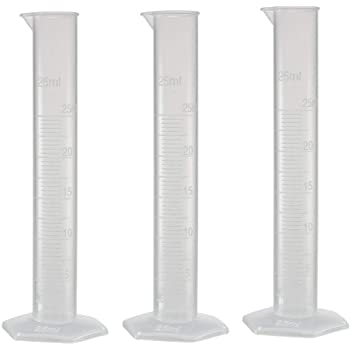
\includegraphics[width=5cm, height=5cm]{cylinders.jpg}
    \caption{Three graduated lab cylinders, corresponding to three
      eigenvectors. Prior eigenvalues not shown.}
    \label{fig:cylinder}
\end{figure}



\section{Clusterization poses no obstruction to D-optimality}\label{section:clusterization}
We saw that the necessary conditions for a design $\obs$ with $m$
observations to be D-optimal are (1), (2) and (4) of Theorem
\ref{thm:char}. As long as these requirements are satisfied, $\obs$ is
D-optimal. These requirements, however, still leave some freedom in
choosing $\obs$. This freedom may give rise to clusterization, as
illustrated in Figure \ref{fig:clusterization} and explained below.

Consider an inverse problem with $\lambda_1^{-1} = 0.1, \lambda_2^{-1}
= 0.2$ and $\sigma^2=1$. In \eqref{eq:two designs}, we suggest two
D-optimal designs $\obs_1, \obs_2$ such that $\obs_1^*\obs_1 =
\obs_2^*\obs_2$. The former exhibits clusterization ($\meas_3 =
\meas_5 = \ev_1$), while the latter does not. Both of these designs
are D-optimal, hence clusterization poses no obstruction to
D-optimality.

\begin{equation}\label{eq:two designs}
  \obs_1 =
  \begin{pmatrix}
    \sqrt{\frac{11}{40}}\ev_1 - \sqrt{\frac{29}{40}}\ev_2 \\
    \sqrt{\frac{11}{40}}\ev_1 + \sqrt{\frac{29}{40}}\ev_2 \\
    \ev_1 \\
    \ev_2 \\
    \ev_1 \\    
  \end{pmatrix},
  \obs_2 =
  \begin{pmatrix}
    \sqrt{\frac{3}{8}}\ev_1 - \sqrt{\frac{5}{8}}\ev_2 \\
    \sqrt{\frac{3}{8}}\ev_1 + \sqrt{\frac{5}{8}}\ev_2 \\
    \sqrt{\frac{2}{5}}\ev_1 - \sqrt{\frac{3}{5}}\ev_2 \\
    \sqrt{\frac{2}{5}}\ev_1 + \sqrt{\frac{3}{5}}\ev_2 \\
    \ev_1 \\    
  \end{pmatrix}
\end{equation}

A computer implementation of Lemma \ref{lemma:free} (see code in
Supplementary material) generates $\obs_1$ as a solution to the
D-optimal design problem mentioned in the previous
paragraph. Modifying the numerical values of the prior does not break
the clusterization. Thus, the preference to clusterization of Lemma
\ref{lemma:free} is robust. The vast majority of randomized numerical
simulations (see code in Supplementary material) also give rise to
D-optimal designs that exhibit clustrization. We conclude that
clusterization poses no obstruction to D-optimality in the relaxed
model presented in this study. Moreover, sensor clusterization is
generic, as far as one accepts the model presented in this study.

%% Of course, a real-life problem is more restricted than the model we
%% consider here. Such restriction is the likely cause of clusterization
%% obseved in, e.g., the toy model of section
%% \ref{subsec:example}. Exactly how this happens is not clear. At this
%% point it is the subject of speculation and should be further studied
%% in the future.

\pgfplotstableread{
  Label    prior  $o_1o_2$  $o_3$   $o_4$   $o_5$    topper
  1         0.1      0.55       1       0       1      0.001
  2         0.2      1.45       0       1       0      0.001
  3         3.5      0          0       0       0      0.001
}\clusterization


\pgfplotstableread{
  Label    prior  $o_1o_2$  $o_3o_4$   $o_5$     topper
  1         0.1    0.75     0.8        1         0.001
  2         0.2    1.25     1.2        0         0.001
  3         3.5    0        0          0         0.001
}\noclusterization

\begin{figure}
  \begin{tikzpicture}[scale=0.85]
    \begin{axis}[
        ybar stacked,
        ymin=0,
        ymax=4,
        xtick=data,
        legend style={cells={anchor=east}, legend pos=north west, legend columns=-1},
        reverse legend=false, % set to false to get correct display, but I'd like to have this true
        xticklabels from table={\clusterization}{Label},
        xticklabel style={text width=2cm,align=center},
        legend plot pos=right,
        ylabel=precision --- prior and posterior,
        xlabel=eigenvector $i$,
      ]
    
      
      \addplot [fill=green!80]  table [y=prior, meta=Label, x expr=\coordindex] {\clusterization};
      \addplot [fill=blue!60]   table [y=$o_1o_2$, meta=Label, x expr=\coordindex] {\clusterization};
      \addplot [fill=red!60]    table [y=$o_3$, meta=Label, x expr=\coordindex] {\clusterization};
      \addplot [fill=black!60]  table [y=$o_4$, meta=Label, x expr=\coordindex] {\clusterization};
      \addplot [fill=orange!60] table [y=$o_5$, meta=Label, x expr=\coordindex] {\clusterization};
      %% \addplot [fill=cyan!60]   table [y=$o_6$, meta=Label, x expr=\coordindex] {\clusterization};
      %% \addplot [fill=purple!60] table [y=$o_7$, meta=Label, x expr=\coordindex] {\clusterization};

      
      \addlegendentry{prior}
      \addlegendentry{$o_1o_2$}
      \addlegendentry{$o_3$}
      \addlegendentry{$o_4$}
      \addlegendentry{$o_5$}
      %% \addlegendentry{$o_6$}
      %% \addlegendentry{$o_7$}   
    \end{axis}
  \end{tikzpicture}
  \qquad
  \begin{tikzpicture}[scale=0.85]
    \begin{axis}[
        ybar stacked,
        ymin=0,
        ymax=4,
        xtick=data,
        legend style={cells={anchor=east}, legend pos=north west, legend columns=-1},
        reverse legend=false, % set to false to get correct display, but I'd like to have this true
        xticklabels from table={\noclusterization}{Label},
        xticklabel style={text width=2cm,align=center},
        legend plot pos=right,
        ylabel=precision --- prior and posterior,
        xlabel=eigenvector $i$,
      ]
    
      
      \addplot [fill=green!80]  table [y=prior, meta=Label, x expr=\coordindex] {\noclusterization};
      \addplot [fill=blue!60]   table [y=$o_1o_2$, meta=Label, x expr=\coordindex] {\noclusterization};
      \addplot [fill=red!60]    table [y=$o_3o_4$, meta=Label, x expr=\coordindex] {\noclusterization};
      \addplot [fill=black!60]  table [y=$o_5$, meta=Label, x expr=\coordindex] {\noclusterization};
      %% \addplot [fill=orange!60] table [y=$o_4$, meta=Label, x expr=\coordindex] {\noclusterization};
      %% \addplot [fill=cyan!60]   table [y=$o_5$, meta=Label, x expr=\coordindex] {\noclusterization};
      %% \addplot [fill=purple!60] table [y=$o_6$, meta=Label, x expr=\coordindex] {\noclusterization};

      
      \addlegendentry{prior}
      \addlegendentry{$o_1o_2$}
      \addlegendentry{$o_3o_4$}
      \addlegendentry{$o_5$}
      %% \addlegendentry{$o_4$}
      %% \addlegendentry{$o_5$}
      %% \addlegendentry{$o_6$}   
    \end{axis}
  \end{tikzpicture}
  \caption{Clusterization (left, $\obs_1$ in \eqref{eq:two designs})
    and non-clusterization (right, $\obs_2$ in \eqref{eq:two designs})
    in D-optimal designs. Posterior precision per eigenvector is
    plotted for $\obs_1$ and $\obs_2$ from \eqref{eq:two
      designs}. Both designs are identical for all practical matters
    --- their posteriors are equal. In the left panel, a D-optimal
    design with clusterization is illustrated: $\meas_3 = \meas_5$. In
    the right panel, a D-optimal design without clusterization is
    illustrated. The contribution to the posterior precision due to
    $\meas_1$ and $\meas_2$ is denoted $\meas_1\meas_2$. These
    contributions are plotted together because $\meas_1$ and $\meas_2$
    are not in the direction of any eigenvector. Similarly for
    $\meas_3\meas_4$.}
  \label{fig:clusterization}
\end{figure}


%% may arise in various scenarios. We first consider
%% sequential designs, and then simultaneous designs.


%% \subsection{Sequential Design}\label{subsec:clusterization sequential}
%% In a sequential optimal design problem, a decision is made on each
%% measurement with all previous measurements fixed. In each step $m=1$,
%% so $k=1$. In this case, Theorem \ref{thm:char} implies each
%% measurement is taken along the direction of the eigenvector of $\fwd
%% \prcov \fwd^*$ with lowest posterior precision. If $\lambda_i$
%% decrease fast enough (e.g. exponentially), then $\lambda_i^{-1}$
%% increase exponentially. Then, at some point, a measurement will be
%% taken along an already measured eigenvector. This situation is
%% measurement clusterization.

%% , $\meas_1 \parallel \ev_1$ and $\eta_1 = 1$. As hinted in
%% section \ref{subsec:seq vs sim}, the posterior becomes the prior for
%% the next step. The eigenvectors of the new posterior are the same as
%% for the previous one. A new observation will be taken in the direction
%% of eigenvector with smalles eigenvalue. This leads to:
%% \begin{align*}
%%   \begin{split}
%%     \meas_2 \parallel \ev_1  &\text{ if } \sigma^2 \lambda^{-1}_1 + 1 < \sigma^2\lambda^{-1}_2 \\
%%     \meas_2 \parallel \ev_2  &\text{ o.w. }
%%   \end{split}
%% \end{align*}
%% In the first case, we get clusterization immediately. In the second,
%% we consider $\meas_3$. Same reasoning leads to the conclusion that the
%% eigenvectors of the new prior precision are the same. The eigenvalues,
%% however, are $\lambda^{-1}_1 + \sigma^{-2}, \lambda^{-1}_2 +
%% \sigma^{-2}, \lambda_3^{-1}, \dots$. A new observation is taken in the
%% direction of eigenvector of smallest precision (note that
%% $\lambda^{-1}_1 + \sigma^{-2} < \lambda^{-1}_2 + \sigma^{-2}$):
%% \begin{align*}
%%   \begin{split}
%%     \meas_3 \parallel \ev_1 &\text{ if } \sigma^2 \lambda^{-1}_1 + 1 <
%%     \sigma^2\lambda^{-1}_3 \\
%%     \meas_3 \parallel  \ev_3  &\text{ o.w. }
%%   \end{split}
%% \end{align*}
%% Again, the first case results in clusterization. The sequential design
%% proceeds in this fashion. Every $\meas_i$ is taken in the direction
%% some eigenvector of the prior $\fwd \prcov\fwd^*$. This eigenvector
%% has the smallest eigenvalue of the previous step's posterior precision
%% operator. If we do not encounter clusterization after $m$ such steps,
%% this means that observation $\meas_k$ was taken in the direction
%% $\ev_k$ for $k=1,\dots,m$. Thus:
%% \begin{align}\label{eq:failure}
%%   \begin{split}
%%     \sigma^2\lambda_{k-1}^{-1} + 1 \geq \sigma^2\lambda_k^{-1}, \text{ for } 1\leq k \leq m
%%     \Longrightarrow \lambda_m^{-1} - \lambda_{m-1}^{-1} \leq \sigma^{-2}.
%%   \end{split}
%% \end{align}

%% But \eqref{eq:failure} implies $\{\lambda_i^{-1}\}_{i=1}^{\infty}$
%% grows at most linearly. In section \ref{subsec:abstract OED} we
%% assumed $\fwd$ is strongly smoothing, which means eigenvalues of
%% $(\fwd \prcov\fwd^*)^{-1}$ grow quickly. Thus, if we take $m$ large
%% enough, \eqref{eq:failure} will eventually fail and we will observe
%% sensor clusterization.


%% \subsection{Simultaneous Design}\label{subsec:clusterization simultaneous}
%% If the eigenvalues $\lambda_i$ decrease quickly enough, we will
%% observe clusterizaion.
